% One-dimensional data
\subsection{One Dimension}
As a very basic proof of concept, we ran the algorithms on the reward
function $r(x) = x$ over the unit interval [0,1].

\begin{figure}[h!]
  \begin{center}
    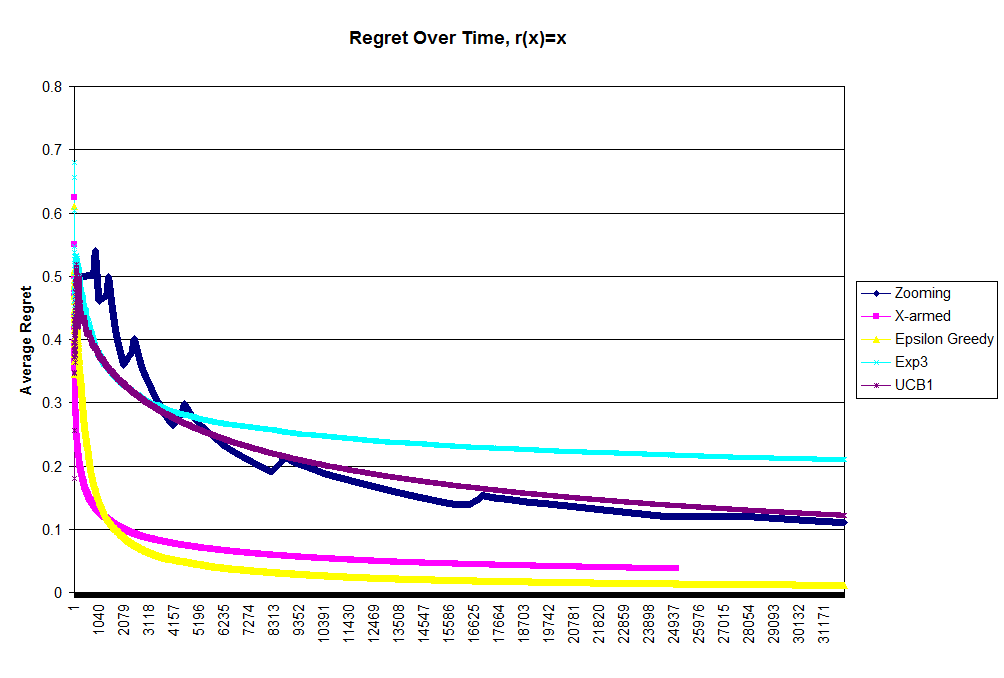
\includegraphics[width=\figwidth]{figures/1dsimpleplot.png}
     \caption{$\epsilon$ r(x) = x, 100 arms for discretization
     algorithms}
     \label{fig:1dsimple}
  \end{center}
\end{figure}

From this plot, we can see a number of facts.  First, at 
least in this case, the $\epsilon$-greedy algorithm is clearly the
best of all discretization algorithms, which is due to there being
no noise.  The $\mathcal{X}$-armed algorithm also does rather well,
but becomes expensive computationally as the number of rounds becomes
large due to having $O(n)$ time complexity in each round, where $t$ is
the number of rounds so far.  We can also see the characteristic bumps of
the Zooming algorithm, which are indicative of the fact that the Zooming
algorithm does not carry over information between phases.

Now we shall add some noise to our reward function.  The new reward
function is $r(x) = b(n_{0,1}(x))$, where $b(x) = 1$ with probability
$x$ and is 0 otherwise and $n_{\alpha_,\beta}(x)$ is $x$ times a random
number uniformly drawn from the interval $[\alpha, \beta]$.